\documentclass[aspectratio=169, pdf, 9pt, utf8]{beamer}
\usepackage[T2A]{fontenc}
\usepackage[utf8]{inputenc}
\usepackage[english,russian]{babel}
\usepackage{amssymb,amsfonts,amsmath,mathtext}
\usepackage{cite,enumerate,float,indentfirst}
\usepackage{booktabs}

\usepackage{multicol}
\graphicspath{{img/}}


\usepackage{pgfplots}
\usepackage{pgfplotstable}
\pgfplotsset{compat = 1.7}

\newcommand{\KG}{\textbf{KaGa}}
\newcommand{\BS}{\textbf{BigSmall}}
\newcommand{\MX}{\textbf{Mix}}
\usetheme{Madrid}
\usecolortheme{whale}

%\setbeamercolor{footline}{fg=gray}
%\setbeamertemplate{footline}{
%  \leavevmode%
%  \hbox{%
%  \begin{beamercolorbox}[wd=.333333\paperwidth,ht=2.25ex,dp=1ex,center]{}%
%    Куликов А.В., ABBYY-MIPT
%  \end{beamercolorbox}%
%  \begin{beamercolorbox}[wd=.333333\paperwidth,ht=2.25ex,dp=1ex,center]{}%
%    Москва, 2017
%  \end{beamercolorbox}%
%  \begin{beamercolorbox}[wd=.333333\paperwidth,ht=2.25ex,dp=1ex,right]{}%
%  Стр. \insertframenumber{} из \inserttotalframenumber \hspace*{2ex}
%  \end{beamercolorbox}}%
%  \vskip0pt%
%}

\usepackage{amsmath}
\DeclareMathOperator*{\argmin}{argmin}
\DeclareMathOperator*{\argmax}{argmax}
\newcommand*{\argminl}{\argmin\limits}
\newcommand*{\argmaxl}{\argmax\limits}

\setbeamerfont{institute}{size=\normalsize}

\newcommand{\itemi}{\item[\checkmark]}

\title[Выпускная квалификационная работа]{Японский: буквенные n-граммы для распознавания}

\author{Куликов Алексей Владимирович}

\vspace{30pt}

\institute[МФТИ]{
	Московский физико-технический институт (государственный университет) \\
	Факультет инновация и высоких технологий \\
	Кафедра компьютерной лингвистики \\
	\vspace{0.5cm}
	Научный руководитель --- А.И. Андрианов
}

\vspace{40pt}

\date{Москва, 2017}

\setbeamertemplate{caption}[numbered]

\begin{document}

\begin{frame}
	\titlepage
\end{frame}

\begin{frame}
	\frametitle{Содержание}
	\tableofcontents
\end{frame}

\section{ Постановка задачи }
\begin{frame}
\frametitle{ Постановка задачи }

\textbf{Цель работы} -- сравнить эффективность различных символьных $n$-граммных моделей в задаче исправления ошибок OCR в японском языке.

Из цели работы вытекают следующие \textbf{задачи:}
\begin{itemize}
	\item Рассмотреть существующие подходы к $n$-граммному моделированию японского языка;
	
	\item Реализовать некоторые символьные $n$-граммные модели;
	
	\item Развернуть систему для тестирования и сравнения моделей.
\end{itemize}
\end{frame}

\begin{frame}
\frametitle{ Формальная постановка задачи }

Формализуем задачу:
\begin{itemize}
	\item {\textit{Алфавит $\Sigma = \{ a, b, c, .. \}$}}.
	
	\item {\textit{Текст $Text \in \Sigma^+$}} делится на конечное число {\textit{предложений $S = \{ S_1, S_2, S_3, ... \}$}} : $Text = S_1S_2S_3...$.
	
	\item Для каждого предложения $S$ существует $k$ вариантов: $S_{set} = \{S_{etalon}, S_{test_1}, ..., S_{test_{k-1}} \}$.
	
	\item {\textit{Оценивающий алгоритм (estimator) $\Theta : S \rightarrow \mathbb{R}^+ $}}.
	
	\item Среди $k$ вариантов предложения выбирается наилучший: $S_{best} = \argmaxl_{S_{set}} \Theta(S)$.
	
	\item {\textit{Качество алгоритма $Q(\Theta) = \dfrac{\#\{ \text{угаданных предложений} \}}{\#\{ \text{всего предложений} \}}$}}.
\end{itemize}

Необходимо сравнить различные алгоритмы по качеству.

\end{frame}

\section{ Модели оценивания текста }

\begin{frame}
	\frametitle{Модели оценивания текста}
	
	\begin{itemize}

\subsection{ Простые n-граммные }
		\item $N$-граммные с фиксированным $n,\ n \in \{1,2,3\}$
			
\subsection{ Backoff-модель }
		\item Backoff-модель, $n_{max} \in \{ 3, 5, 7 \}$
		
		\[ P_n(w_i | w_{i - n + 1}, ..., w_{i - 1}) =
		\begin{cases}
		C(w_i | w_{i - n + 1}, ..., w_{i - 1})       & \quad \text{if } C(w_i | w_{i - n + 1}, ..., w_{i - 1}) > k\\
		P_{n - 1}(w_i | w_{i - n + 2}, ..., w_{i - 1})  & \quad \text{otherwise }\\
		\end{cases}
		\]

\subsection{ Модель Катца (Katz) }		
		\item Модель Катца (Katz),  $n_{max} \in \{ 3, 5, 7 \}$
		
		\[
		P_{n}\left( w_i | w_{i-n+1}...w_{i-1} \right) = 
		\begin{cases}
		d_{w_{i-n+1}...w_i} \dfrac{C(w_{i-n+1}...w_i)}{C(w_{i-n+1}...w_{i-1})} &\text{if $C(w_{i-n+1}...w_i) > k$}\\
		\alpha_{w_{i-n+1}...w_{i-1}} P_{n - 1}\left( w_i | w_{i-n+2}...w_{i-1} \right) &\text{otherwise}
		\end{cases}
		\]
		
	\end{itemize}

\end{frame}

\section{ Описание эксперимента }

\subsection{ Корпус }

\begin{frame}
	\frametitle{Корпус}
	
	
	HTML-страницы с различных японских сайтов, 163244 штуки.
	
	Статистики по корпусу после его обработки:
	
	\begin{table}[H]
		\begin{center}
			\begin{tabular}{|l|c|} \hline
				Параметр & Значение \\ \hline 
				Размер (kB) & 1 721 504 \\
				Символов & 640 604 961 \\
				среди них уникальных & 6 861 \\
				Предложений & 79 497 345	\\  \hline
			\end{tabular}
			\caption{Характеристики корпуса}
			\label{table:corpora}
		\end{center}
	\end{table}
\end{frame}

\begin{frame}
	\frametitle{Количество униграмм}
	
	\begin{multicols}{2}
			\begin{center}
			
			\begin{figure}[H]
				\begin{tikzpicture}
				\begin{axis}
				[
				height=6cm,
				%ybar,
				%bar width=20pt,
				ylabel={Количество, шт},
				xlabel={Порядковый номер символа},
				axis x line=bottom,
				axis y line=left,
				enlarge x limits=0.1,
				enlarge y limits=0.1,
				]	
				\addplot gnuplot[raw gnuplot, mark=none, color=blue]{ plot 'plots/1gramstats.csv' using ($1):($2) every 5 with lines; };
				\end{axis}
				\end{tikzpicture}
				\caption{Распределение частот униграмм}
				\label{plt:gramstats1_all}
			\end{figure}
		\end{center}
	
	\begin{center}
		
		\begin{figure}[H]
			\begin{tikzpicture}
			\begin{axis}
			[
			height=6cm,
			%ybar,
			%bar width=20pt,
			ylabel={Количество, шт},
			xlabel={Порядковый номер символа},
			axis x line=bottom,
			axis y line=left,
			enlarge x limits=0.1,
			enlarge y limits=0.1,
			]	
			\addplot gnuplot[raw gnuplot, mark=none, color=blue]{ plot 'plots/1gramstats.csv' using ($1):($2) every 5::::200 with lines; };
			\end{axis}
			\end{tikzpicture}
			\caption{Частоты униграмм -- голова распределения }
			\label{plt:gramstats1_head}
		\end{figure}
	\end{center}
	\end{multicols}
	
\end{frame}

\subsection{ Buckets }
\begin{frame}
	\frametitle{Buckets}
	{\textit{Корзина (бакет, bucket)}} -- множество символов, которые считаются статистически малозначимыми и заменяются на U+FFFD (Unicode Replacement Character).
	
	Выбран бакет с $|\Sigma_{B^*}| = 4800$.
	
	\begin{center}
		
		\begin{figure}[H]
			\begin{tikzpicture}
			\begin{axis}
			[
		height=6cm,
			%ybar,
			%bar width=20pt,
			ylabel={Количество, шт},
			xlabel={Порядковый номер символа},
			axis x line=bottom,
			axis y line=left,
			enlarge x limits=0.1,
			enlarge y limits=0.1,
			]	
			\addplot gnuplot[raw gnuplot, only marks, color=blue]{ plot 'plots/1gramstats-bucket.csv' using ($1):($2) every 5 with lines; };	\addplot gnuplot[raw gnuplot, only marks, color=red]{ plot 'plots/1gramstats-bucketed.csv' using ($1):($2) every 5 with lines; };
			\end{axis}
			\end{tikzpicture}
			\caption{Распределение частот униграмм: бакет с $|\Sigma_{B_i}| = 2600$}
			\label{fig:bucket_pic}
		\end{figure}
		
	\end{center}
\end{frame}

\subsection{ Шум как эмуляция ошибок OCR }

\begin{frame}
	\frametitle{Шум как эмуляция ошибок OCR}
	
	Необходимо эмулировать ошибки OCR.
	
	\begin{itemize}
		\item \textbf{KaGa}
		
		\begin{center}
			\begin{figure}[H]
				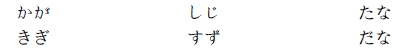
\includegraphics[height=30pt]{p_KG.png}
			\end{figure}
		\end{center}
		
		\item \textbf{BigSmall}
			\begin{center}
			\begin{figure}[H]
				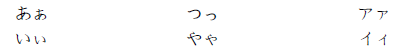
\includegraphics[height=30pt]{p_BS.png}
			\end{figure}
		\end{center}
		
		\item \textbf{Mix}
			\begin{center}
			\begin{figure}[H]
				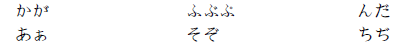
\includegraphics[height=30pt]{p_MX.png}
			\end{figure}
		\end{center}
	\end{itemize}
\end{frame}

\begin{frame}
	\frametitle{Пример шума}
	
	\begin{center}
		\begin{figure}[H]
			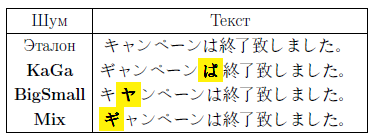
\includegraphics{p_noise.png}
		\end{figure}
	\end{center}
\end{frame}

\begin{frame}
	\frametitle{Распределение шумов по униграммам}
	
	\begin{center}
	\begin{figure}[H]
		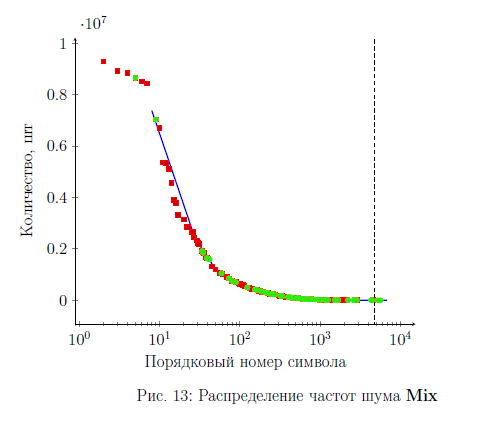
\includegraphics[height=7cm]{p_ndistr.png}
	\end{figure}
\end{center}
\end{frame}

\subsection{ Baseline }

\begin{frame}
	Униграммная модель.
	
	Результаты показаны для основного бакета, $|\Sigma_{B^*}| = 4800$.
	
	\begin{table}[H]
		\begin{center}
			\begin{tabular}{|c|c|} \hline
				Шум 	& Оценка модели \\ \hline
				\textbf{KaGa}	& 0.75  \\
				\textbf{BigSmall} & 0.88  \\
				\textbf{Mix} & 0.76 \\ \hline
			\end{tabular}
			\caption{Baseline}
			\label{table:baseline}
		\end{center}
	\end{table}
	
\end{frame}

\subsection{ Сравнение моделей }
\section{ Результаты эксперимента }

\begin{frame}
	\frametitle{Результаты}
	
	\begin{table}[H]
		\begin{center}
			
			\begin{tabular}{|c|c|c|c|}\hline
				$M \backslash N$ & \KG & \BS & \MX \\ \hline
				Ngram(1) (Baseline) & 0.75 & 0.88 & 0.76 \\
				Backoff(5) & 0.89 & 0.93 & 0.90 \\
				Katz(5) & 0.961 & 0.965 & 0.962 \\ \hline 	
			\end{tabular}
			\caption{Результаты эксперимента: accuracy}
			\label{table:exp1}
		\end{center}
	\end{table}
\end{frame}

\section{ Результаты эксперимента -- уверенность }

\begin{frame}
	\frametitle{Результаты -- уверенность}
	
	\begin{table}[H]
		\begin{center}
			
			\begin{multicols}{2}
				\begin{tabular}{|c|c|c|c|}\hline
					$C \backslash N$ & \KG & \BS & \MX \\ \hline
					0.9 & 0.86 & 0.94 & 0.86 \\
					0.95 & 0.979 & 0.988 & 0.981 \\
					0.97 & 0.966  & 0.986 & 0.967  \\
					0.99 & 0.94 & 0.98 & 0.95 \\ \hline 	
				\end{tabular}
				\caption*{Accuracy}
				
				\begin{tabular}{|c|c|c|c|}\hline
					$C \backslash N$ & \KG & \BS & \MX \\ \hline
					0.9 & 0.53 & 0.43 & 0.52 \\
					0.95 & 0.61 & 0.69 & 0.62 \\
					0.97 & 0.77 & 0.85  & 0.77  \\
					0.99 & 0.91 & 0.94 & 0.91 \\ \hline 	
				\end{tabular}
				\caption*{Доля классифицированных}
			\end{multicols}		
			\caption{Результаты эксперимента c $Confidence$}
			\label{table:exp1}
		\end{center}
	\end{table}

Выбрана модель Katz($n=5, C=0.97$).
\end{frame}

\subsection{ Статистика по n-граммам }
\begin{frame}
	\frametitle{Статистика по $n$-граммам}
	
		\begin{center}
		\begin{figure}[H]
			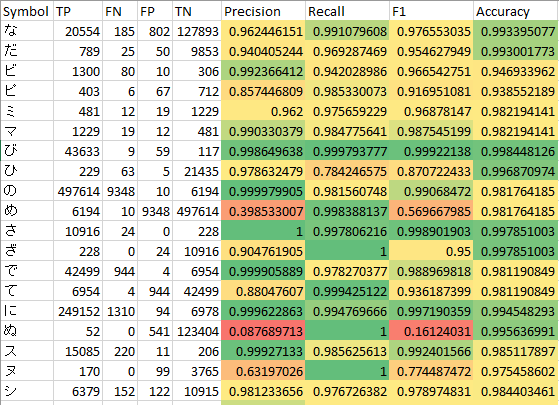
\includegraphics[height=7cm]{p_stats.png}
		\end{figure}
	\end{center}
	
\end{frame}

\begin{frame}
	\frametitle{Ресурсы}
	
	
	\begin{table}[H]
		\begin{center}
			\begin{tabular}{|c|c|c|} \hline
				Модель & Место на диске & RAM \\ \hline
				1-gram & 100 KB & $\approx$ 1 MB \\
				3-gram trie &  178 MB & $\approx$ 7 MB \\
				5-gram trie &  1.5 GB & $\approx$ 40 GB \\
				7-gram trie & 3.7 GB & $\approx$ 110 GB \\ \hline
			\end{tabular}
			\caption{Затраты ресурсов, память, $|\Sigma| = 4800$}
			\label{table:resmem}
		\end{center}
	\end{table}
	
	\begin{table}[H]
		\begin{center}
			\begin{tabular}{|c|c|c|} \hline
				Модель & 10000 примеров & 1000000 примеров \\ \hline
				1-gram & $<$ 1 мин & $\approx$ 20 мин \\
				3-gram trie &  $\approx$ 1 мин  & $\approx$ 1.5 ч \\
				5-gram trie &  $\approx$ 2 мин & $\approx$ 3 ч \\ \hline
			\end{tabular}
			\caption{Затраты ресурсов, время, $|\Sigma| = 4800$}
			\label{table:restime}
		\end{center}
	\end{table}
\end{frame}
\section{ Анализ результатов эксперимента }

\subsection{ Сравнение с другими результатами }

\begin{frame}
	\frametitle{Сравнение с другими результатами}
	
	Работа Nagata, использующая backoff $n$-граммы для исправления ошибок OCR.
	
	Также использует размеченный корпус со словным делением.
	
	\begin{table}[H]
		\begin{center}
			
			\begin{tabular}{|c|c|}\hline
				Модель & Accuracy \\ \hline
				Katz			 &  0.96--0.986 \\
				Nagata & 0.97--0.98 \\ \hline 	
			\end{tabular}
			\caption{Сравнение с результатами Nagata}
			\label{table:nagres}
		\end{center}
	\end{table}
	
\end{frame}


\subsection{ Анализ ошибок }

\begin{frame}
	\frametitle{Анализ ошибок}
	
	Нехватка информации в $n$-граммной модели.
	
	Существуют примеры, которые модель незаслуженно трактует как неверные.
			\begin{center}
		\begin{figure}[H]
			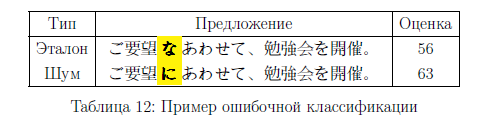
\includegraphics{p_err.png}
		\end{figure}
	\end{center}
\end{frame}

\begin{frame}
	\frametitle{Использованное ПО}
	
	\begin{itemize}
		\item Python 3.5.2 (pickle, dot, nltk, unicodedammit)
		
		\item Bash
		
		\item Graphviz
	\end{itemize}
\end{frame}


\begin{frame}
\center{\Huge
%	ありがとう
Спасибо
}
\end{frame}

\end{document} 